\section{Boxplots}


\begin{figure}[htbp]
	\centering
	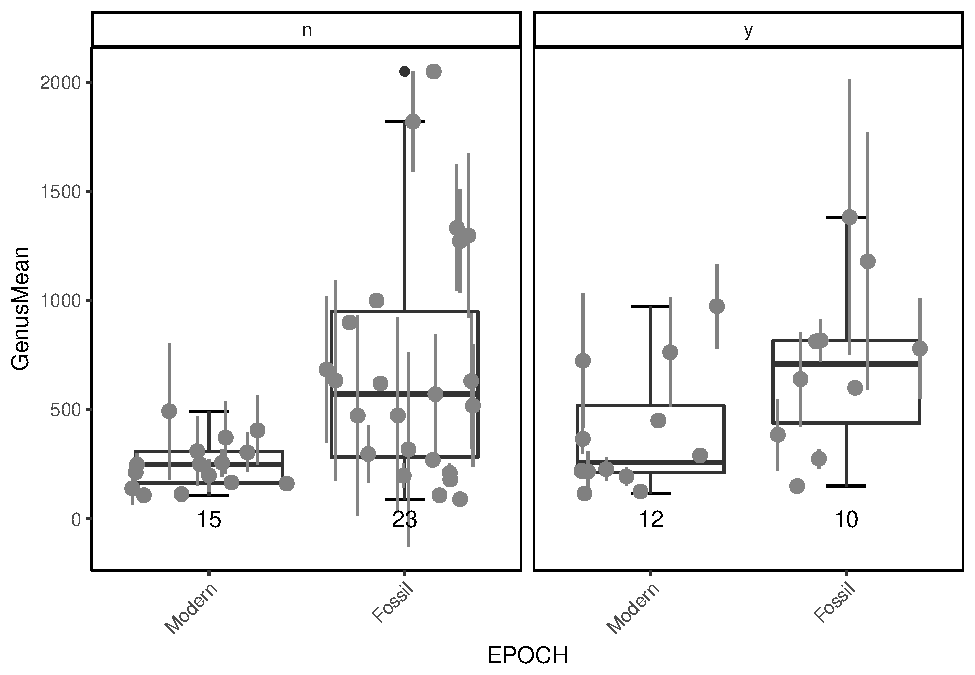
\includegraphics{MA_JJ_files/figure-latex/BPFMCI-1.pdf}
	\caption{Boxplots fossil vs.~modern, continental vs.~insular species.}
	\label{BoxFoMCI}
\end{figure}


Wilcoxon Rank Sum Test (unpaired data):

modern continental \textless{} fossil continental (P =
\(4.8532266\times 10^{-8}\))

modern insular \textless{} fossil insular (P = \(0.0018564\))
%Kruskal-Wallis-Test:

%Continent means differ (P = \(1.0833256\times 10^{-6}\)) (still have to
%look into the details\ldots{})

\begin{figure}[htbp]
	\centering
	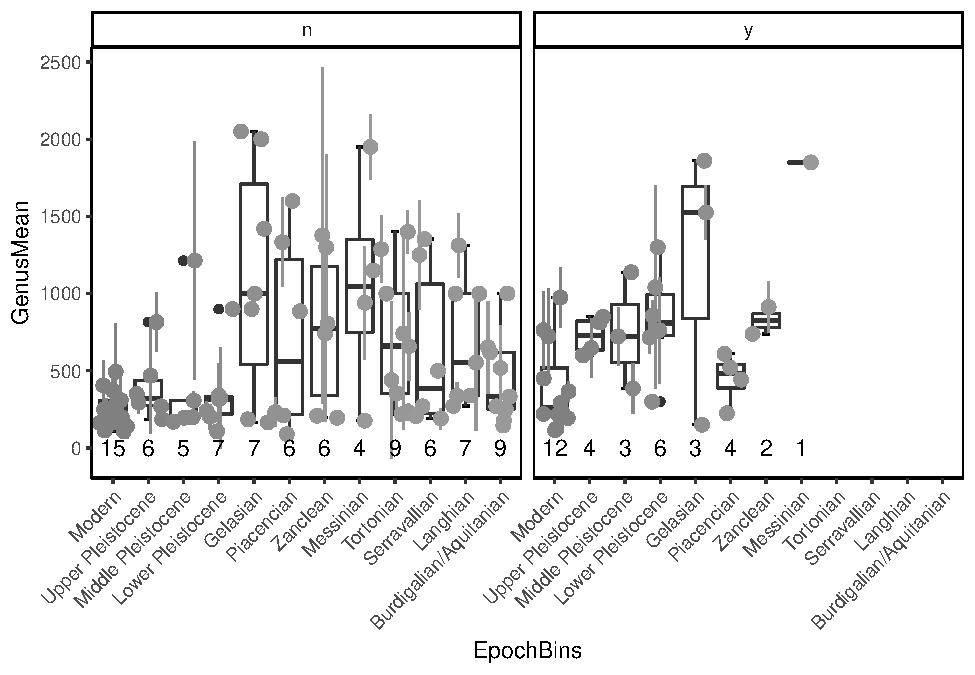
\includegraphics{MA_JJ_files/figure-latex/Box_FM_timebin.pdf}
	\caption{Boxplots time bins, continental vs.~insular species.}
	\label{BoxTBCI}
\end{figure}


%no longer in R-Script, look in old scripts, if it should stay here!!!

% continental
%Multiple comparison test after Kruskal-Wallis 
%p.value: 0.05 
%Comparisons
%obs.dif critical.dif difference
%Modern-Upper Pleistocene                  15.0333333     41.09142      FALSE
%Modern-Middle Pleistocene                  5.2666667     43.92857      FALSE
%Modern-Lower Pleistocene                   8.7952381     38.93852      FALSE
%Modern-Gelasian                           32.7238095     38.93852      FALSE
%Modern-Piacencian                         20.0333333     41.09142      FALSE
%Modern-Zanclean                           27.0333333     41.09142      FALSE
%Modern-Messinian                          32.8666667     47.87005      FALSE
%Modern-Tortonian                          29.2555556     35.86753      FALSE
%Modern-Serravallian                       20.3666667     41.09142      FALSE
%Modern-Langhian                           30.7238095     38.93852      FALSE
%Modern-Burdigalian/Aquitanian             14.7555556     35.86753      FALSE
%Upper Pleistocene-Middle Pleistocene       9.7666667     51.51082      FALSE
%Upper Pleistocene-Lower Pleistocene        6.2380952     47.32708      FALSE
%Upper Pleistocene-Gelasian                17.6904762     47.32708      FALSE
%Upper Pleistocene-Piacencian               5.0000000     49.11364      FALSE
%Upper Pleistocene-Zanclean                12.0000000     49.11364      FALSE
%Upper Pleistocene-Messinian               17.8333333     54.91071      FALSE
%Upper Pleistocene-Tortonian               14.2222222     44.83441      FALSE
%Upper Pleistocene-Serravallian             5.3333333     49.11364      FALSE
%Upper Pleistocene-Langhian                15.6904762     47.32708      FALSE
%Upper Pleistocene-Burdigalian/Aquitanian   0.2777778     44.83441      FALSE
%Middle Pleistocene-Lower Pleistocene       3.5285714     49.81032      FALSE
%Middle Pleistocene-Gelasian               27.4571429     49.81032      FALSE
%Middle Pleistocene-Piacencian             14.7666667     51.51082      FALSE
%Middle Pleistocene-Zanclean               21.7666667     51.51082      FALSE
%Middle Pleistocene-Messinian              27.6000000     57.06489      FALSE
%Middle Pleistocene-Tortonian              23.9888889     47.44828      FALSE
%Middle Pleistocene-Serravallian           15.1000000     51.51082      FALSE
%Middle Pleistocene-Langhian               25.4571429     49.81032      FALSE
%Middle Pleistocene-Burdigalian/Aquitanian  9.4888889     47.44828      FALSE
%Lower Pleistocene-Gelasian                23.9285714     45.47039      FALSE
%Lower Pleistocene-Piacencian              11.2380952     47.32708      FALSE
%Lower Pleistocene-Zanclean                18.2380952     47.32708      FALSE
%Lower Pleistocene-Messinian               24.0714286     53.31876      FALSE
%Lower Pleistocene-Tortonian               20.4603175     42.86990      FALSE
%Lower Pleistocene-Serravallian            11.5714286     47.32708      FALSE
%Lower Pleistocene-Langhian                21.9285714     45.47039      FALSE
%Lower Pleistocene-Burdigalian/Aquitanian   5.9603175     42.86990      FALSE
%Gelasian-Piacencian                       12.6904762     47.32708      FALSE
%Gelasian-Zanclean                          5.6904762     47.32708      FALSE
%Gelasian-Messinian                         0.1428571     53.31876      FALSE
%Gelasian-Tortonian                         3.4682540     42.86990      FALSE
%Gelasian-Serravallian                     12.3571429     47.32708      FALSE
%Gelasian-Langhian                          2.0000000     45.47039      FALSE
%Gelasian-Burdigalian/Aquitanian           17.9682540     42.86990      FALSE
%Piacencian-Zanclean                        7.0000000     49.11364      FALSE
%Piacencian-Messinian                      12.8333333     54.91071      FALSE
%Piacencian-Tortonian                       9.2222222     44.83441      FALSE
%Piacencian-Serravallian                    0.3333333     49.11364      FALSE
%Piacencian-Langhian                       10.6904762     47.32708      FALSE
%Piacencian-Burdigalian/Aquitanian          5.2777778     44.83441      FALSE
%Zanclean-Messinian                         5.8333333     54.91071      FALSE
%Zanclean-Tortonian                         2.2222222     44.83441      FALSE
%Zanclean-Serravallian                      6.6666667     49.11364      FALSE
%Zanclean-Langhian                          3.6904762     47.32708      FALSE
%Zanclean-Burdigalian/Aquitanian           12.2777778     44.83441      FALSE
%Messinian-Tortonian                        3.6111111     51.11909      FALSE
%Messinian-Serravallian                    12.5000000     54.91071      FALSE
%Messinian-Langhian                         2.1428571     53.31876      FALSE
%Messinian-Burdigalian/Aquitanian          18.1111111     51.11909      FALSE
%Tortonian-Serravallian                     8.8888889     44.83441      FALSE
%Tortonian-Langhian                         1.4682540     42.86990      FALSE
%Tortonian-Burdigalian/Aquitanian          14.5000000     40.10112      FALSE
%Serravallian-Langhian                     10.3571429     47.32708      FALSE
%Serravallian-Burdigalian/Aquitanian        5.6111111     44.83441      FALSE
%Langhian-Burdigalian/Aquitanian           15.9682540     42.86990      FALSE


% insular
%Multiple comparison test after Kruskal-Wallis 
%p.value: 0.05 
%Comparisons
%obs.dif critical.dif difference
%Modern-Upper Pleistocene                  10.0833333     19.92445      FALSE
%Modern-Middle Pleistocene                  9.8333333     22.27622      FALSE
%Modern-Lower Pleistocene                  12.3333333     17.25508      FALSE
%Modern-Gelasian                           12.5000000     22.27622      FALSE
%Modern-Piacencian                          1.8333333     19.92445      FALSE
%Modern-Zanclean                           13.8333333     26.35757      FALSE
%Modern-Messinian                          22.8333333     35.91932      FALSE
%Modern-Tortonian                                 NaN          Inf         NA
%Modern-Serravallian                              NaN          Inf         NA
%Modern-Langhian                                  NaN          Inf         NA
%Modern-Burdigalian/Aquitanian                    NaN          Inf         NA
%Upper Pleistocene-Middle Pleistocene       0.2500000     26.35757      FALSE
%Upper Pleistocene-Lower Pleistocene        2.2500000     22.27622      FALSE
%Upper Pleistocene-Gelasian                 2.4166667     26.35757      FALSE
%Upper Pleistocene-Piacencian               8.2500000     24.40237      FALSE
%Upper Pleistocene-Zanclean                 3.7500000     29.88668      FALSE
%Upper Pleistocene-Messinian               12.7500000     38.58354      FALSE
%Upper Pleistocene-Tortonian                      NaN          Inf         NA
%Upper Pleistocene-Serravallian                   NaN          Inf         NA
%Upper Pleistocene-Langhian                       NaN          Inf         NA
%Upper Pleistocene-Burdigalian/Aquitanian         NaN          Inf         NA
%Middle Pleistocene-Lower Pleistocene       2.5000000     24.40237      FALSE
%Middle Pleistocene-Gelasian                2.6666667     28.17743      FALSE
%Middle Pleistocene-Piacencian              8.0000000     26.35757      FALSE
%Middle Pleistocene-Zanclean                4.0000000     31.50333      FALSE
%Middle Pleistocene-Messinian              13.0000000     39.84891      FALSE
%Middle Pleistocene-Tortonian                     NaN          Inf         NA
%Middle Pleistocene-Serravallian                  NaN          Inf         NA
%Middle Pleistocene-Langhian                      NaN          Inf         NA
%Middle Pleistocene-Burdigalian/Aquitanian        NaN          Inf         NA
%Lower Pleistocene-Gelasian                 0.1666667     24.40237      FALSE
%Lower Pleistocene-Piacencian              10.5000000     22.27622      FALSE
%Lower Pleistocene-Zanclean                 1.5000000     28.17743      FALSE
%Lower Pleistocene-Messinian               10.5000000     37.27524      FALSE
%Lower Pleistocene-Tortonian                      NaN          Inf         NA
%Lower Pleistocene-Serravallian                   NaN          Inf         NA
%Lower Pleistocene-Langhian                       NaN          Inf         NA
%Lower Pleistocene-Burdigalian/Aquitanian         NaN          Inf         NA
%Gelasian-Piacencian                       10.6666667     26.35757      FALSE
%Gelasian-Zanclean                          1.3333333     31.50333      FALSE
%Gelasian-Messinian                        10.3333333     39.84891      FALSE
%Gelasian-Tortonian                               NaN          Inf         NA
%Gelasian-Serravallian                            NaN          Inf         NA
%Gelasian-Langhian                                NaN          Inf         NA
%Gelasian-Burdigalian/Aquitanian                  NaN          Inf         NA
%Piacencian-Zanclean                       12.0000000     29.88668      FALSE
%Piacencian-Messinian                      21.0000000     38.58354      FALSE
%Piacencian-Tortonian                             NaN          Inf         NA
%Piacencian-Serravallian                          NaN          Inf         NA
%Piacencian-Langhian                              NaN          Inf         NA
%Piacencian-Burdigalian/Aquitanian                NaN          Inf         NA
%Zanclean-Messinian                         9.0000000     42.26615      FALSE
%Zanclean-Tortonian                               NaN          Inf         NA
%Zanclean-Serravallian                            NaN          Inf         NA
%Zanclean-Langhian                                NaN          Inf         NA
%Zanclean-Burdigalian/Aquitanian                  NaN          Inf         NA
%Messinian-Tortonian                              NaN          Inf         NA
%Messinian-Serravallian                           NaN          Inf         NA
%Messinian-Langhian                               NaN          Inf         NA
%Messinian-Burdigalian/Aquitanian                 NaN          Inf         NA
%Tortonian-Serravallian                           NaN          Inf         NA
%Tortonian-Langhian                               NaN          Inf         NA
%Tortonian-Burdigalian/Aquitanian                 NaN          Inf         NA
%Serravallian-Langhian                            NaN          Inf         NA
%Serravallian-Burdigalian/Aquitanian              NaN          Inf         NA
%Langhian-Burdigalian/Aquitanian                  NaN          Inf         NA


